%
% chapter.tex
%
% (c) 2020 Prof Dr Andreas Müller
%
\chapter{Lineare Gleichungssysteme\label{chapter:linsys}}
\lhead{Lineare Gleichungssysteme}
\rhead{}
Die lineare Algebra ist fundamental in vielen Bereichen der angewandeten
Mathematik.
Eine grosse Zahl von Methoden zur Lösung linearer
Gleichungssysteme, zur Zerlegung von Matrizen und zur Lösung des
Eigenwertproblems sind über die Jahrhunderte entwickelt worden und
werden zum Teil bereits in Anfängervorlesungen unterrichtet.
Insbesondere der Gausssche Elminitationsalgorithmus gehört zu den
grundlegenden Techniken der numerischen linearen Algebra, wird hier
aber als bekannt vorausgesetzt.

Die meisten Techniken gehen von relativ kleinen Gleichungssystemen aus.
Sie sind aber schlicht nicht leistungsfähig genug oder stabil genug für 
grosse Systeme, wie sie zum Beispiel bei der Lösung von partiellen
Differentialgleichungen oder Simulationen komplexer Systeme auftreten.
Auch ist die Laufzeit für die exakte Lösung oft zu lang.
Zum Beispiel hat der Gauss-Algorithmus für $n$ Unbekannte Laufzeitkomplexität
$O(n^3)$, was für Gleichungsyssteme mit $n>10^5$ zu prohitiv grossem
Aufwand führt.
Kompromisse zwischen exakter Lösung und Durchführbarkeit in vernünftiger
Zeit sind daher unumgänglich.
Bereits Gauss hat daher iterative numerische Methoden entwickelt.

Dieses Kapitel präsentiert einige wenige Algorithmen des überaus weiten
Feldes der numerischen linearen Algebra, welche die Vielfalt dieses
Gebietes illustrieren sollen.
Eine vertiefte Darstellung kann gefunden werden in \cite{buch:watkins}.
In Abschnitt~\ref{buch:section:gaussseidel} wird gezeigt, wie sich
Gleichungssysteme unter gewissen Voraussetzungen auch iterativ lösen
lassen.
Die QR-Zerlegung ist eine andere Formulierung des Problems, eine Basis
zu orthonormalisieren, welches schon vom Gram-Schmidt-Algorithmus gelöst
wurde, welcher allerdings gewisse Stabilitätsprobleme hat.
Der in Abschnitt~\ref{buch:section:qr} vorgestellte, auf Spiegelungen
basierende Algorithmus ist effizienter und stabiler.
Das Eigenwertproblem für symmetrische Matrizen ist von grundlegender
Bedeutung für die Anwendungen, die Lösung über das charakteristische 
Polynom, welches man oft in den Grundlagenvorlesungen lernt, ist jedoch
nur für sehr kleine Matrizen praktikabel.
Abschnitt~\ref{buch:section:jacobi} stellt das Jacobi-Verfahren zur
Diagonalisierung symmetrischer Matrizen vor, welches ebenfalls iterativ
arbeitet.

Weitere Verfahren der numerischen linearen Algebra werden in einzelnen
Artikeln des zweiten Teiles vorgetellt.

%
% thomas.tex
%
% (c) 2020 Prof Dr Andreas Müller, Hochschule Rapperswil
%
\section{Direkte Verfahren
\label{buch:section:direkt}}
\rhead{Direkte Verfahren}
Das primäre direkte Verfahren zur Lösung linearer Gleichungssysteme ist
der Gauss-Algorithmus, der allerdings
zur Lösung linearer Gleichungssysteme im Allgemeinen $O(n^3)$
Operationen braucht, was für grosse $n$ zu aufwendig ist.
\index{Gauss-Algorithmus}%

%
% XXX Formelzusammenstellung für den Gauss-Algorithmus
%

\subsection{Thomas-Algorithmus für tridiagonale Matrizen
\label{buch:subsection:thomasalgorithmus}}
Es gibt einen Fall, der zum Beispiel bei der Diskretisierung
partieller Differentialgleichungen mit nur einer Raumdimension
häufig auftritt, nämlich der Fall {\em tridiagonaler} Koeffizientenmatrix.
\index{tridiagonal}%
Dies sind Matrizen der Form
\begin{equation}
A
=
\begin{pmatrix}
b_1   & c_1   &  0    &  0    &\dots  &  0    &  0     \\
a_2   & b_2   & c_2   &  0    &\dots  &  0    &  0     \\
 0    & a_3   & b_3   & c_3   &\dots  &  0    &  0     \\
 0    &  0    & a_4   & b_4   &\ddots &  0    &  0     \\
\vdots&\vdots &\vdots &\ddots &\ddots &\ddots &\vdots  \\
 0    &  0    &  0    &  0    &\ddots &b_{n-1}&c_{n-1} \\
 0    &  0    &  0    &  0    &\dots  &a_{n}  &b_n
\end{pmatrix},
\end{equation}
deren Einträge alle $0$ sind ausser auf der Diagonalen und den unmittelbar
benachbarten Nebendiagonalen.
\index{Nebendiagonale}%
Eine solche Matrix enstand auch im
Abschnitt~\ref{buch:subsection:splineinterpolant}
bei der Bestimmung der Steigungen für die Spline-Interpolationsfunktion.
\index{Spline-Interpolationsfunktion}%

Da die meisten Einträge der Matrix verschwinden, geben nur die wenigstens
Zeilenoperationen des Gauss-Algorithmus überhaupt etwas zu tun.
Dadurch sinkt der Aufwand für die Durchführung des Algorithmus.
\index{Gauss-Algorithmus}%
\index{Zeilenoperation}%

\subsubsection{Vorwärtsreduktion}
Die Vorwärtsreduktion entfernt die Element unter der Diagonalen
und macht die Pivotelemente zu $1$.
\index{Vorwärtsreduktion}%
\index{Pivotelement}%
Man muss also nur herausfinden, wie sich die Elemente $c_i$ über der
Diagonalen verändern.
Bei der Vorwärtsreduktion wird das ursprüngliche Gauss-Tableau daher
wie folgt umgewandelt:
\index{Gauss-Tableau}%
\[
\begin{tabular}{|>{$}c<{$}>{$}c<{$}>{$}c<{$}>{$}c<{$}>{$}c<{$}>{$}c<{$}|>{$}c<{$}|}
\hline
b_1   & c_1  &  0   &  0   &  0   &\dots & d_1  \\
a_2   & b_2  & c_2  &  0   &  0   &\dots & d_2  \\
 0    & a_3  & b_3  & c_3  &  0   &\dots & d_3  \\
 0    &  0   & a_4  & b_4  & c_4  &\dots & d_4  \\
\vdots&\vdots&\vdots&\vdots&\vdots&\ddots&\vdots\\
\hline
\end{tabular}
\to
\begin{tabular}{|>{$}c<{$}>{$}c<{$}>{$}c<{$}>{$}c<{$}>{$}c<{$}>{$}c<{$}|>{$}c<{$}|}
\hline
 1    & c_1' &  0   &  0   &  0   &\dots & d_1' \\
 0    &  1   & c_2' &  0   &  0   &\dots & d_2' \\
 0    &  0   &  1   & c_3' &  0   &\dots & d_3' \\
 0    &  0   &  0   &  1   & c_4' &\dots & d_4' \\
\vdots&\vdots&\vdots&\vdots&\vdots&\ddots&\vdots\\
\hline
\end{tabular}
\]
mit
\begin{equation}
c_i
=
\begin{cases} 
\displaystyle \frac{c_1\mathstrut}{b_1\mathstrut}            &\quad i=1\\[8pt]
\displaystyle \frac{c_i\mathstrut}{b_i-a_ic'_{i-1}\mathstrut}&\quad i>1
\end{cases}
\qquad\text{und}\qquad
d_i
=
\begin{cases}
\displaystyle\frac{d_1\mathstrut}{b_1\mathstrut}                        &\quad i=1\\[8pt]
\displaystyle\frac{d_i-a_id'_{i-1}\mathstrut}{b_i-a_ic'_{i-1}\mathstrut}&\quad i>1
\end{cases}
\label{buch:equation:thomasvorwaerts}
\end{equation}
Die Vorwärtsreduktion ist also mit $O(n)$ Operationen durchführbar.

\begin{beispiel}
In der Matrix
\begin{equation}
A=\begin{pmatrix}
    -2&     1&     0&     0&     0&\dots \\
     1&    -2&     1&     0&     0&\dots \\
     0&     1&    -2&     1&     0&\dots \\
     0&     0&     1&    -2&     1&\dots \\
     0&     0&     0&     1&    -2&\ddots\\
\vdots&\vdots&\vdots&\vdots&\ddots&\ddots
\end{pmatrix}
\label{buch:equation:Atridiagonal}
\end{equation}
gilt $a_i=1$, $b_i=-2$ und $c_i=1$ für alle $i$.
Aus den Formeln~\eqref{buch:equation:thomasvorwaerts}
folgt dann
\begin{align*}
c_1'&=-\frac12
\\
c_2'&=\frac{1}{-2-c_1'}=\frac{1}{-2+\frac12}=-\frac{2}{3}
\\
c_3'&=\frac{1}{-2-c_2'}=\frac{1}{-2+\frac{2}{3}}=\frac{3}{-2\cdot 3 + 2}
=-\frac{3}{4}.
\end{align*}
Daraus lässt sich vermuten, dass
\begin{equation}
c_k'=-\frac{k}{k+1}
\label{buch:equation:ck}
\end{equation}
gilt.
Tatsächlich lässt sich dies mit vollständiger Induktion beweisen.
\index{vollständige Induktion}%
Zunächst ist $c_1=-\frac12=-\frac1{1+1}$ korrekt.
Jetzt muss man zeigen, dass aus der Formel \eqref{buch:equation:ck} für $k$
die Formel für $k+1$ folgt.
Durch nachrechnen sieht man, dass
\[
c_{k+1}'
=
\frac1{-2-c_{k}'}
=
\frac{1}{-2+\displaystyle\frac{k}{k+1}}
=
\frac{k+1}{-2(k+1)+k}
=
-\frac{k+1}{k+2}.
\]
Damit ist \eqref{buch:equation:ck} bewiesen.

Wir führen die Vorwärtsreduktion für einen Vektor aus lauter Einsen
als rechte Seite durch, also $d_i=1$.
\index{Vorwärtsreduktion}%
Die Formeln \eqref{buch:equation:thomasvorwaerts} gibt dann
\begin{align*}
d_1'
&=
\frac{d_1}{b_1} = -\frac12
\\
d_2'
&=
\frac{1-d_1'}{-2-c_1'}
=
\frac{\frac32}{-2+\frac12}
=
\frac{\frac32}{-\frac{3}{2}}
=-1
\\
d_3'
&=
\frac{1-d_2'}{-2+c_2'}
=
\frac{1+1}{-2+\frac23}
=
\frac{2\cdot 3}{-2\cdot 3 + 2}
=
-\frac{3}{2}.
\end{align*}
Aus diesen Werten lässt sich wieder die Vermutung 
\[
d_{k}'=-\frac{k}2
\]
ableiten.
Und tatsächlich beweist die Rechnung
\[
d_{k+1}'
=
\frac{1-d_k'}{-2+\frac{k}{k+1}}
=
\frac{1+\frac{k}{2}}{-2+\frac{k}{k+1}}
=
\frac{1+\frac{k}{2}}{-2(k+1)+k} (k+1)
=
\frac{k+2}{-2k-2+k}
\cdot
\frac{k+1}{2}
=
\frac{k+2}{-k-2}
\cdot
\frac{k+1}{2}
=
-\frac{k+1}{2}
\]
diese Vermutung mit vollständiger Induktion.
\end{beispiel}

\subsubsection{Rückwärtseinsetzen}
\index{Rückwärtseinsetzen}%
Das Rückwärtseinsetzen ist jetzt ebenfalls sehr einfach:
\begin{equation}
x_k = \begin{cases}
d_n'&\quad k=n
\\
d_k'  - c_k' x_{k+1} &\quad k < n
\end{cases}
\label{buch:equation:rueckwaerts}
\end{equation}
Auch das Rückwärtseinsetzen ist daher mit $O(n)$ Operationen machbar.
Der Thomas-Algorithmus löst also ein tridiagonales Gleichungssystem in
\index{Thomas-Algorithmus}%
$O(n)$ Operationen oder berechnet die inverse Matrix einer 
tridiagonalen Matrix in $O(n^2)$ Operationen.

\begin{beispiel}
Für die Matrix $A$ von \eqref{buch:equation:Atridiagonal} und die rechte
Seite von Einsen aus dem entsprechenden Beispiel  können wir jetzt auch
das Rückwärtseinsetzen durchführen.
Dazu wenden wir die Formeln
\eqref{buch:equation:rueckwaerts}
auf die oben gefundenen Werte $c'_k=-k/(k+1)$ und $d_k'=-k/2$ an und
erhalten
\begin{align*}
x_n
&=
-\frac{n}{2}
&&=\frac{1\cdot (n-0)}2
\\
x_{n-1}
&=
-\frac{n-1}{2} -\biggl(-\frac{n-1}{n}\biggr)\cdot \biggl(-\frac{n}2\biggr)
=
-\frac{n-1}{2} - \frac{n-1}{2}
=
-(n-1)
&&=-\frac{2(n-1)}{2}
\\
x_{n-2}
&=
-\frac{n-2}{2} - \biggl(-\frac{n-2}{n-1}\biggr) \cdot (-n+1)
=
-\frac{n-2}{2} - (n-2)
=
-\frac{3(n-2)}2
&&=-\frac{3(n-2)}2
\\
x_{n-3}
&=
-\frac{n-3}{2} - \frac{n-3}{n-2} \frac{3(n-2)}2
=
-\frac{n-3}{2} - 3\frac{n-3}2
=
\frac{4(n-3)}2
&&=-\frac{4(n-3)}2
\end{align*}
woraus man die Vermutung
\begin{equation}
x_{n-k} = -\frac{(k+1)(n-k)}2
\label{buch:equation:xn}
\end{equation}
ableiten.
Tatsächlich rechnet man nach
\begin{align*}
x_{n-(k+1)}
=
d_{n-(k+1)}'-c_{n-(k+1)}'x_{n-k}
&=
-\frac{n-(k+1)}2-\frac{n-k-1}{n-k}\cdot \frac{(k+1)(n-k)}2
\\
&=
-\frac{n-(k+1)+(n-k-1)(k+1)}2
\\
&=
-\frac{(k+2)(n-(k+1))}2.
\end{align*}
Damit ist die Formel für $x_n$ bewiesen.

Man kann natürlich auch direkt verifizieren, dass die $x_k$ das tridiagonale
Gleichungssystem lösen:
\begin{align*}
x_{n-(k-1)}-2x_{n-k} + x_{n-(k+1)}
&=
-\frac{
k(n-(k-1))
-2(k+1)(n-k)
+(k+2)(n-(k+1))
}2
\\
&=
-\frac{
kn-k^2+k
-2kn-2n+2k^2+2k
+kn+2n-k^2-3k-2}2=1.
\end{align*}
Dies gilt auch für $k=0$  und $k=n-1$, weil die Formel~\eqref{buch:equation:xn}
\[
x_{n+1}=x_{n-(-1)} = -\frac{(-1+1)(n-(-1))}2=0
\qquad\text{und}\qquad
x_0 = x_{n-n} = -\frac{(n+1)(n-n)}2
\]
zur Folge hat.
\end{beispiel}

\subsection{Zyklisch tridiagonale Matrix
\label{buch:subsection:zyklischtridiagonal}}
Die Diskretisation des Poisson-Problems oder der Wärmeleitungsgleichung
auf einem Ring liefert eine tridiagonale Matrix, in der zusätzlich die
Einträge in den Ecken links unten und rechts oben von $0$ verschieden sind.
\index{Poisson-Problem}%
\index{Matrix!tridiagonal}%
\index{tridiagonale Matrix}%
Bei der Durchführung des Gauss-Algorithmus werden damit zusätzliche 
Einträge im Tableau von $0$ verschieden sein, so dass zusätzliche Operationen
notwendig werden:
\index{Gauss-Algorithmus}%
\index{Tableau}%
\begin{itemize}
\item 
Zusätzlich zu der Zeilenoperation, die die Element 
$a_i$ zu $0$ macht braucht es jeweils noch eine Operation, welche das
Element in der letzten Zeile annihiliert.
\index{Zeilenoperation}%
Dadurch wird aber ein neuer nicht verschwindender Eintrag erzeugt,
so dass eine Operation für jedes Element der letzten Zeile nötig wird,
also $O(n)$ zusätzliche Operation.
\item
Die Zeilenoperationen erzeugen aus dem Element in der rechten oberen
Ecke nicht verschwindende Elemente in der Spalte ganz recht.
Beim Rückwärtseinsetzen sind daher im ersten Schritt $O(n)$ 
zusätzliche Operatione notwendig.
\end{itemize}
Auch ein Gleichungssystem mit zyklisch tridiagonaler Matrix lässt sich also 
mit $O(n)$ Operationen lösen und die Matrix lässt sich mit $O(n^2)$
Operationen invertieren.

Tatsächlich erfordert das Invertieren einer Matrix nur $O(n^2)$
zusätzliche Operationen, wenn die Inverse einer Matrix bereits
bekannt ist, die sich in nur einer Stelle unterscheidet.
Dies ist der Inhalt der Sherman-Morrison-Woodbury-Formel, die
im nächsten Abschnitt untersucht wird.

\subsection{Sherman-Morrison-Woodbury-Formel
\label{buch:subsection:sherman-morrison-woodbury-formel}}
\index{Sherman-Morrison-Woodbury-Formel}%
Eine zyklisch tridiagonale Matrix unterscheidet sich nur in zwei 
Positionen von einer tridiagonalen Matrix.
Diese kleine Änderung verdoppelt den Rechenaufwand für die Lösung
des Gleichungssystems.
Es stellt sich die Frage, ob sich eine Matrix auf billige Art
ändern lässt derart, dass die Invertierung mit dem weniger
aufwendigen Thomas-Algorithmus möglich wird.
\index{Thomas-Algorithmus}%
Die {\em Sherman-Morrison-Woodbury-Formel} 

\begin{satz}[Shermann-Morrison-Woodburry]
\label{buch:satz:shermann}
Ist $A$ eine Matrix mit der Inversen $A^{-1}$ und sind die Vektoren
$u$ und $v$ gegeben derart, dass $v^tA^{-1}u\ne 1$ ist, dann gilt
\begin{equation}
(A-uv^t)^{-1}
=
A^{-1} + \frac{1}{1-v^tA^{-1}u} A^{-1}uv^tA^{-1}.
\label{buch:equation:shermann-morrison-woodburry}
\end{equation}
\end{satz}

\begin{proof}[Beweis]
Wir schreiben 
\[
B
=
A^{-1} + \frac{1}{1-v^tA^{-1}u} A^{-1}uv^tA^{-1}
\]
für die rechte Seite der
Formel \eqref{buch:equation:shermann-morrison-woodburry}.
Wir beweisen die Behauptung durch Nachrechnen.
Den Ausdruck $v^tA^{-1}u$ kürzen wir im Folgenden $c$ ab.
Es gilt
\begin{align*}
(A-uv^t)
B
&=
(A-uv^t)
\biggl(
A^{-1} + \frac{1}{1-v^tA^{-1}u} A^{-1}uv^tA^{-1}
\biggr)
\\
&=
AA^{-1}-uv^tA^{-1}
+
\frac{1}{1-c}
\biggl(
AA^{-1}uv^tA^{-1}
-u\underbrace{v^tA^{-1}u}_{\displaystyle=c}v^tA^{-1}
\biggr)
\\
&=
E-uv^tA^{-1}
+
\frac{1}{1-c}
\biggl(
uv^t
-cu v^t
\biggr)A^{-1}
\\
&=
E-uv^tA^{-1}
+
uv^t
A^{-1}
=
E.
\qedhere
\end{align*}
\end{proof}

\begin{beispiel}
Die Matrix
\[
A
=
\begin{pmatrix}
-2& 1& 0& 0& 0\\
 1&-2& 1& 0& 0\\
 0& 1&-2& 1& 0\\
 0& 0& 1&-2& 1\\
 0& 0& 0& 1&-2
\end{pmatrix}
\qquad
\text{und}
\qquad
B
=
\begin{pmatrix}
-2& 1& 0& 0& 0\\
 1&-2& 1& 0& 0\\
 0& 1&-2& 1& 0\\
 0& 0& 1&-2& 1\\
{\color{red} 1}& 0& 0& 1&-2
\end{pmatrix}
\]
unterscheiden sich nur durch ein einziges Element in der linken unteren
Ecke.
Dieses Element kann betrachtet werden als ein Produkt von
Standardbasisvektoren
\index{Standardbasisvektor}%
\[
E_{51}
=
\begin{pmatrix}
 0& 0& 0& 0& 0\\
 0& 0& 0& 0& 0\\
 0& 0& 0& 0& 0\\
 0& 0& 0& 0& 0\\
 1& 0& 0& 0& 0
\end{pmatrix}
=
e_5e_1^t.
\]
Ausserdem ist $A^{-1}$ mit Hilfe des Thomas-Algorithmus leicht berechenbar,
\index{Thomas-Algorithmus}%
sie ist
\[
\renewcommand\arraystretch{1.15}
A^{-1}
= 
\begin{pmatrix}
-\frac56 & -\frac23 & -\frac12 & -\frac13 & -\frac16 \\
-\frac23 & -\frac43 & -1       & -\frac23 & -\frac13 \\
-\frac12 & -1       & -\frac32 & -1       & -\frac12 \\
-\frac13 & -\frac23 & -1       & -\frac43 & -\frac23 \\
-\frac16 & -\frac13 & -\frac12 & -\frac23 & -\frac56
\end{pmatrix}.
\]
Um Satz~\ref{buch:satz:shermann} anzuwenden, müssen wir $B=A-uv^t$ schreiben.
Dies gelingt mit $u=-e_5$ und $v=e_1$.
Die Formel~\eqref{buch:equation:shermann-morrison-woodburry} ist nur dann
anwendbar, wenn $v^tA^{-1}u\ne 1$ ist, wir rechnen daher nach und finden
$c=v^tA^{-1}u=\frac16$.
Damit kann jetzt die Inverse von $B$ bestimmt werden:
\begin{align*}
B^{-1}
&=
(A-uv^t)^{-1}
=
A^{-1} + \frac65 A^{-1}uv^tA^{-1}
=
\renewcommand\arraystretch{1.15}
\begin{pmatrix}
-1& -\frac45 & -\frac35 & -\frac25 & -\frac15 \\
-1& -\frac85 & -\frac65 & -\frac45 & -\frac25 \\
-1& -\frac75 & -\frac95 & -\frac65 & -\frac35 \\
-1& -\frac65 & -\frac75 & -\frac85 & -\frac45 \\
-1& -1       & -1       & -1       & -1       
\end{pmatrix}.
\qedhere
\end{align*}
\end{beispiel}

Man beachte, dass sich jede Matrix mit Rang $1$ in der Form $uv^t$
schreiben lässt.
%Ist $C$ eine Matrix mit Rang $1$, dann sind alle Vektoren $Cx$
%Vielfache eines einzigen Vektors $u$.
Da $\operatorname{Rang}C=1$ ist, hat der Nullraum $N=\operatorname{ker}C$
von $C$ die Dimension $n-1$ und es gibt einen Einheitsvektor $v$,
der orthogonal auf allen Vektoren des Nullraumes ist.
Jeder Vektor $x\in \mathbb R^n$ kann zerlegt werden in
$x=x_{\|} + x_{\perp}$ mit $x_{\perp}\in\operatorname{ker}C$ und
$x_{\|}=v(v\cdot x)=v v^tx$, es gilt dann
$Cx = Cx_{\|} + Cx_{\perp} = Cx_{\|}$.
Setzen wir $u=Cv$, dann folgt wegen $x_{\|} = v(v\cdot x)$ 
\[
Cx = Cx_{\|} = Cv v^t x = uv^t x
\qquad\Rightarrow\qquad
C = uv^t.
\]
Satz~\ref{buch:satz:shermann} besagt daher, dass die Inverse einer
Matrix $B$, die sich nur um eine Matrix vom Rang $1$ von $A$ unterschiedet,
mit Rechenaufwand $O(n^2)$ aus der Inversen $A^{-1}$ ermittelt werden kann.
Dies bringt allerdings nur einen Nutzen, wenn der Aufwand zur Berechung
von \eqref{buch:equation:shermann-morrison-woodburry} geringer ist als
eine volle Durchführung des Gauss-Algorithmus.
\index{Gauss-Algorithmus}%
Dazu beachtet man, dass ein Produkt $\text{Matrix}\times\text{Vektor}$ 
mit $O(n^2)$ Operationen möglich ist.
Sowohl $A^{-1}u$ und $v^tA^{-1}$ lassen sich daher mit $O(n^2)$
Operationen bestimmen.
Das Produkt des Spaltenvektors $A^{-1}u$ mit dem Zeilenvektor $v^tA^{-1}$
ist sogar in $O(n)$ Operationen möglich.
\index{Spaltenvektor}%
\index{Zeilenvektor}%
Auf diese Weise lässt sich
die Formel~\ref{buch:equation:shermann-morrison-woodburry} mit
$O(n^2)$ Operationen durchführen und ist daher weniger aufwändig als
der Gauss-Algorithmus.
 
\subsection{Bandmatrizen}
\index{Bandmatrix}%
Tridiagonale Matrizen waren einfach zu invertieren, weil es nur wenige
von $0$ verschiedene Einträge nahe der Diagonalen gab.
\index{Diagonale}%
Diese Bedingung erfüllen auch sogenannte {\em Bandmatrizen}.
Eine $n\times n$-Matrix $A$ mit Einträgen $a_{ij}$ ist eine Bandmatrix
der Breite $k$, wenn $a_{ij} = 0$ für $|i-j|>k$.
\begin{figure}
\centering
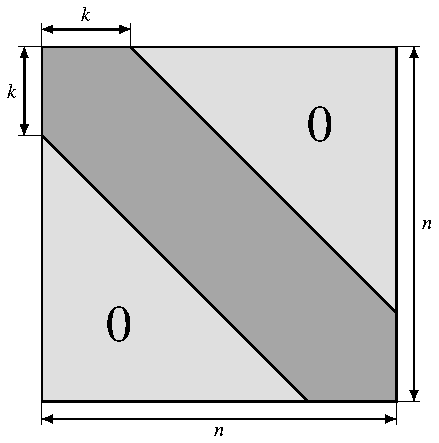
\includegraphics{chapters/60-linsys/images/bandmatrix.pdf}
\caption{Eine Bandmatrix ist eine $n\times n$-Matrix, deren Einträge
ausserhalb eines Bandes um die Diagonale verschwinden.
\index{Band}%
\label{buch:figure:bandmatrix}}
\end{figure}
Schematisch kann man eine solche Matrix wie in
Abbildung~\ref{buch:figure:bandmatrix} darstellen.

Der Gauss-Algorithmus braucht auch in einer Bandmatrix nicht die
volle Zahl von Operationen.
Bei der Pivotdivision müssen höchstens $2k+1$ Divisionen ausgeführt
werden.
\index{Pivotdivision}%
Danach sind genau $k$ Zeilenoperationen notwendig, um die Spalte
unter dem Pivotelement zu $0$ zu machen.
\index{Zeilenoperation}%
Dabei werden nur die Elemente in $2k+1$ Spalten modifiziert,
der Aufwand für jeden Schritt der Vorwärtsreduktion ist daher $(k^2)$.
\index{Vorwärtsreduktion}%
Nach $n$ Schritten wurde daher Rechenzeit $O(nk^2)$ aufgewendet.
\index{Rechenzeit}%
Beim Rückwärtseinsetzen werden in $n$ Iteration jeweils $k$ Zeilenoperationen
in genau zwei Spalten durchgeführt, es fallen also nur $O(nk)$
Operationen an.
\index{Rückwärtseinsetzen}%
Insgesamt sind also nur $O(nk^2)$ Operationen nötig, um ein Gleichungssystem
zu lösen, oder $O(n^2k^2)$ für eine Matrixinvertierung.
\index{Matrixinvertierung}%

Die Diskretisation einer partiellen Differentialgleichung in der Ebene
\index{partielle Differentialgleichung}%
\index{Differentialgleichung!partiell}%
mit finiten Differenzen
\index{finite Differenzen}%
(siehe auch Abschnitt~\ref{section:finite-differenzen})
führt auf natürlich Weise zu einem linearen
Gleichungssystem mit einer Bandmatrix mit $k\approx \sqrt{n}$.
Ein solches Gleichungssystem lässt sich mit Aufwand $O(n^2)$ statt 
$O(n^3)$ lösen.








%
% gausseidel.tex
%
% (c) 2020 Prof Dr Andreas Müller, Hochschule Rapperswil
%
\section{Iterative Gleichungslösung
\label{buch:section:gaussseidel}}
\rhead{Gauss-Seidel-Iteration}
\index{Gleichungssystem!linear}%
\index{lineares!Gleichungssystem}%
Gegeben ist eine lineares Gleichungssystem von $n$ Gleichungen mit
$n$ Unbekannten, welches wir als
\begin{equation}
\begin{linsys}{5}
a_{11}x_1 &+& a_{12}x_2 &+& \dots  \hspace*{7pt}&+& a_{1n}x_n &=& b_1 \\
a_{21}x_1 &+& a_{22}x_2 &+& \dots  \hspace*{7pt}&+& a_{2n}x_n &=& b_2 \\
\vdots\hspace*{5pt}  & & \vdots\hspace*{5pt}  & & \ddots \hspace*{7pt}& & \vdots\hspace*{5pt}  & & \vdots\hspace*{5pt} \\
a_{21}x_1 &+& a_{n2}x_2 &+& \dots  \hspace*{7pt}&+& a_{nn}x_n &=& b_n
\end{linsys}
\label{buch:eqn:linalg:system}
\end{equation}
schreiben.
Abgekürzt wird das Gleichungssystem auch $Ax=b$ notiert, wobei $A=(a_{ij})$
die Koeffizientenmatrix ist, $x=(x_k)$ der Vektor der Unbekannten
und $b=(b_k)$ der Vektor der rechten Seiten.
\index{Koeffizientenmatrix}%

%
% Iterative Lösung
%
\subsection{Iterative Lösung nach Gauss-Seidel
\label{buch:subsection:gauss-seidel}}
Jede der Gleichungen \eqref{buch:eqn:linalg:system} kann nach jeder Variablen
aufgelöst werden, deren zugehöriger Koeffizient von $0$ verschieden ist.
Die Gleichung $k$ in \eqref{buch:eqn:linalg:system} ist
\[
a_{k1}x_1 + a_{k2}x_2 + \dots + a_{kk}x_k + \dots a_{kn}x_n = b_k
\]
Aufgelöst nach $x_k$ ist dies
\[
{\color{red}x_k}
=
\frac1{a_{kk}} (b_k - a_{k1}x_1 - a_{k2}x_2 - \dots - a_{kn}x_n),
\]
sofern $a_{kk}\ne 0$.
Diese Gleichung kann dazu verwendet werden, die Werte für die Unbekannten
zu verbessern.
Wir verwenden daher die Notation $x^{(m)}$ für die $m$-te Approximation
der Lösung.

\begin{satz}[Gauss-Seidel-Iteration]
\index{Gauss-Seidel-Iteration}%
Unter geeigneten Voraussetzungen konvergiert die Folge $x^{(m)}$
definiert durch
\begin{equation}
{\color{red}x_k^{(m)}}
=
\frac{1}{a_{kk}}\bigl(
b_k  - a_{k1}x_1^{(m)} - \dots - a_{k,k-1}x_{k-1}^{(m)}
- a_{k,k+1}x_{k+1}^{(m-1)} - \dots - a_{kn}x_n^{(m-1)}
\bigr)
\label{buch:eqn:gs:iteration}
\end{equation}
mit Startwert $x^{(0)}=0$
gegen die Lösung $x$ des Gleichungssystems $Ax=b$.
\end{satz}

In Abschnitt~\ref{buch:subsection:konvergenzbedingung} werden die
Bedingungen genauer untersucht, die Konvergenz des Verfahrens gegen die
Lösung garantieren können.
\index{Konvergenzbedingung}%

\begin{beispiel}
Sei das Gleichungssystem gegeben durch
\begin{equation}
A=\begin{pmatrix}
2&1&1\\
1&3&1\\
1&1&4
\end{pmatrix}
\qquad\text{und}\qquad
b=\begin{pmatrix}
7\\6\\5
\end{pmatrix}.
\label{buch:eqn:gsbeispiel}
\end{equation}
Die Berechnung der Folge $x^{(m)}$ nach
\eqref{buch:eqn:gs:iteration}
liefert die Werte in Tabelle~\ref{buch:table:gaussseidelbeispiel}.
Die Konvergenz scheint linear zu sein.
\begin{table}
\centering
\begin{tabular}{|>{$}r<{$}|>{$}r<{$}>{$}r<{$}>{$}r<{$}|}
\hline
 m & x_1^{(m)} & x_2^{(m)} & x_3^{(m)} \\
\hline
 0 & 0.0000000             & 0.0000000             & 0.0000000             \\
 1 & 3.5000000             & 0.8333333             & 0.1666667             \\
 2 & 3.0000000             & 0.9444444             & 0.2638889             \\
 3 & \underline{2.8}958333 & \underline{0.94}67593 & \underline{0.2}893519 \\
 4 & \underline{2.88}19444 & \underline{0.94}29012 & \underline{0.29}37886 \\
 5 & \underline{2.88}16552 & \underline{0.941}5187 & \underline{0.294}2065 \\
 6 & \underline{2.882}1373 & \underline{0.941}2187 & \underline{0.2941}610 \\
 7 & \underline{2.8823}102 & \underline{0.94117}62 & \underline{0.2941}284 \\
 8 & \underline{2.8823}476 & \underline{0.94117}47 & \underline{0.29411}94 \\
 9 & \underline{2.882353}1 & \underline{0.94117}59 & \underline{0.294117}7 \\
10 & \underline{2.882353}1 & \underline{0.9411764} & \underline{0.2941176} \\
\hline
\infty&   2.8823529 & 0.9411764 & 0.2941176 \\
\hline
\end{tabular}
\caption{Lösung des Gleichungssystems mit Koeffizientenmatrix $A$ und
rechter Seite $b$ aus \eqref{buch:eqn:gsbeispiel} mit Hilfe des
Gauss-Seidel-Algorithmus.
\index{Gauss-Seidel-Algorithmus}%
In der letzten Zeile die exakten Resultate, erhalten mit dem
Gauss-Algorithmus.
\index{Gauss-Algorithmus}%
\label{buch:table:gaussseidelbeispiel}}
\end{table}
\end{beispiel}


%
% Matrixformulierung
%
\subsection{Matrixformulierung
\label{buch:subsection:matrixformulierung}}
Die Iterationsformel~\eqref{buch:eqn:gs:iteration} verknüpft bei der
Berechnung von $\color{red}x^{(m)}$ Komponenten von $x^{(m-1)}$ und
$\color{red}x^{(m)}$,
\index{Iterationsformel}%
was es etwas schwieriger macht, die Iteration als Fixpunktiteration
der Form ${\color{red}x^{(m)}} = Fx^{(m-1)}$ mit einer
$n\times n$-Matrix $F$ zu schreiben.
\index{Fixpunktiteration}%
\index{Iteration}%
Um dies zu erreichen, zerlegen wir die Matrix $A$ in drei Summanden
$A=L+D+U$, wobei $L$ eine untere Dreiecksmatrix mit Nullen auf der 
Diagonalen sein soll, $D$ eine Diagonalmatrix und $U$ eine obere
Dreiecksmatrix mit  Nullen auf der Diagonalen, also
\begin{align*}
L
&=
\begin{pmatrix}
0        &0        &0        &\dots   & 0         & 0      \\
a_{21}   &0        &0        &\dots   & 0         & 0      \\
a_{31}   &a_{3,2}  &0        &\dots   & 0         & 0      \\
\vdots   &\vdots   &\ddots   &\ddots  & \vdots    & \vdots \\
a_{n-1,1}&a_{n-1,2}&a_{n-1,3}&\dots   & 0         & 0      \\
a_{n1}   &a_{n2}   &a_{n3}   &\dots   & a_{n,n-1} & 0
\end{pmatrix},
\qquad
U
=
\begin{pmatrix}
0      & a_{12} & \dots  & a_{1,n-2} & a_{1,n-1}   & a_{1n} \\
0      & 0      & \dots  & a_{1,n-2} & a_{2,n-1}   & a_{2n} \\
\vdots & \vdots & \ddots & \ddots    &\vdots       & \vdots \\
0      & 0      & \dots  & 0         & a_{n-2,n-1} & a_{n-2,n} \\
0      & 0      & \dots  & 0         & 0           & a_{n-1,n} \\
0      & 0      & \dots  & 0         & 0           & 0
\end{pmatrix}
\intertext{und}
D
&=
\operatorname{diag} (a_{11}, a_{22},\dots , a_{n-1,n-1}, a_{nn}).
\end{align*}
Die Iterationsformel~\eqref{buch:eqn:gs:iteration} lässt sich
mit diesen Matrizen schreiben als
\[
D{\color{red}x^{(m)}} = b - L{\color{red}x^{(m)}} - Ux^{(m-1)}.
\]
Auflösen nach $x^{(m)}$ führt auf
\begin{equation}
{\color{red}x^{(m)}} = (D+L)^{-1} ( b - Ux^{(m-1)} ).
\label{buch:eqn:gs:fixpunkt}
\end{equation}
Die Form \eqref{buch:eqn:gs:fixpunkt} für das Gauss-Seidel-Iterationsverfahren
ist jetzt die einer Fixpunkt-Iteration.

%
% Konvergenzbedingung
%
\subsection{Konvergenzbedingung
\label{buch:subsection:konvergenzbedingung}}
In Kapitel~\ref{chapter:berechnung} haben wir gelernt, dass eine
Fixpunktiteration konvergiert, wenn der Betrag der Ableitung $<1$ ist.
Hier liegt jedoch eine Matrix-Iteration mit der Abbildung
\[
F(x)
=
\underbrace{(D+L)^{-1} b}_{\displaystyle=c} - (D+L)^{-1}U x
=
c - (D+L)^{-1}Ux
\]
vor.
Die Ableitung ist daher ebenfalls eine Matrix, nämlich
\[
D_xF = (D+L)^{-1}U,
\]
und der Fehler der Iteration $m$ ist
\begin{equation}
\delta_m = (D+L)^{-1}U \delta_{m-1}.
\label{buch:gs:fehler}
\end{equation}
Konvergenz kann also nur vorliegen, wenn dieser Vektor im Laufe der
Iteration immer kleiner wird.
\index{Konvergenz}%
Dies ist zum Beispiel dann der Fall, wenn die {\em Norm} der Matrix
kleiner als $1$ ist:
\index{Norm}%

\begin{definition}
Die {\em Norm} einer Matrix $M$ ist
\[
\|M\|
=
\max\{|Mx|\,|\, x\in\mathbb R^n\wedge |x|=1\}.
\]
Für einen Vektor $x\in\mathbb R^n$ gilt $|Mx| \le \|M\|\cdot |x|$.
\end{definition}

Die Bedingung \eqref{buch:gs:fehler} bedeutet jedoch nicht,
dass die Norm der Ableitung $<1$ sein muss, es genügt, wenn
genügend hohe Potenzen der Ableitung eine Norm $<1$ haben.
\index{Ableitung}%

\begin{beispiel}
Die Matrix
\[
M=\begin{pmatrix}
0&2\\
\frac13&0
\end{pmatrix}
\]
hat Norm
\[
\|M\|
=
\max_{|x|=1} |Mx| 
=
\max_{t\in\mathbb R} \sqrt{2^2\cos^2 t +\frac1{3^2}\sin^2t} \ge 2.
\]
Da aber
\[
M^2 = \begin{pmatrix}
\frac{2}{3}&0\\
0&\frac{2}{3}
\end{pmatrix}
\qquad\Rightarrow\qquad \|M^2\|=\frac23
\]
ist, wird eine Iteration mit Ableitungsmatrix $M$ trotzdem
konvergieren, weil der Fehler nach jedem zweiten Schritt um den
Faktor $\frac23$ kleiner geworden ist.
\end{beispiel}

Dies führt uns auf die Grösse
\begin{equation}
\pi(M)
=
\limsup_{n\to\infty} \|M^n\|^\frac1n.
\label{buch:eqn:gelfand-grenzwert}
\end{equation}
Ist $\pi(M) > 1$, dann gibt es Anfangsvektoren $v$ für die Iteration,
für die $M^kv$ über alle Grenzen wächst.
Ist $\pi(M) < 1$, dann wird jeder Anfangsvektor $v$ zu einer Iterationsfolge
$M^kv$ führen, die gegen $0$ konvergiert.
Die Kennzahl $\pi(M)$ erlaubt also zu entscheiden, ob ein
Iterationsverfahren konvergent ist.
\index{Konvergenzbedingung}%

Die Berechnung von $\pi(M)$ als Grenzwert ist sehr unhandlich.
Viel einfacher ist der Begriff des Spektralradius.
\index{Spektralradius}%

\begin{definition}
\label{buch:definition:spektralradius}
Der {\em Spektralradius} der Matrix $M$ ist der Betrag des betragsgrössten
Eigenwertes.
\end{definition}

Wir werden später in Satz~\ref{buch:satz:gelfand} zeigen, dass
$\pi(M) = \varrho(M)$, dies ist bekannt als der Satz von Gelfand.
Um die beiden Begriffe bis dann auseinander halten zu können,
nennen wir den Grenzwert~\ref{buch:eqn:gelfand-grenzwert}
den {\em Gelfand-Radius} $\pi(M)$ der Matrix $M$.
\index{Gelfand-Radius}%
Wir erlauben uns aber, die Überlegungen zu den Iterationsverfahren
mit dem Spektralradius zu formulieren.

Das Gauss-Seidel-Iterationsverfahren ist also genau dann für alle
Startwerte $x_0$ linear konvergent, wenn der Spektralradius
\[
\varrho\bigl( (L+D)^{-1}U \bigr) < 1
\]
ist.
\index{Iterationsverfahren}%

\subsection{Zerlegungsverfahren
\label{buch:subsection:zerlegung}}
\index{Zerlegungsverfahren}%
Das Gauss-Seidel-Verfahren ist nur ein Beispiel einer ganzen Familie
von iterativen Lösungsverfahren für lineare Gleichungssysteme.
Sie basieren alle auf einer Zerlegung $A=B+C$ der Matrix $A$.
Das Gauss-Seidel-Verfahren ist der Fall
\[
A = \underbrace{D+L}_{\displaystyle = B} + \underbrace{R}_{\displaystyle = C}.
\]
Das ursprüngliche Gleichungssystem $Ax=b$ wird jetzt ebenfalls
aufgeteilt in $Bx+Cx=b$.
Ein iteratives Verfahren ergibt sich jetzt dadurch, dass für die beiden $x$
in der Aufteilung verschiedene Iterationen der Lösung verwendet werden,
also $Bx^{(m+1)} + Cx^{(m)} = b$.
Wir erhalten somit das Iterationsverfahren
\begin{equation}
{\color{red}x^{(m+1)}}
=
B^{-1}(b-Cx^{(m)})
=
b_0 - B^{-1}Cx^{(m)}
\end{equation}
Dies ist natürlich nur sinnvoll, wenn sich die Matrix $B$ wesentlich
leichter invertieren lässt als $A$, da andernfalls die Bestimmung von
$x^{(m+1)}$ nicht einfacher ist als die Lösung des ursprünglichen
Gleichungssystems.

Iteriert wird also die Anwendung der Matrix $B^{-1}C$.
Aus der oben entwickelten Theorie lesen wir ab, dass das Zerlgungsverfahren
genau dann konvergiert, wenn der Spektralradius 
$\varrho(B^{-1}C)$ von $B^{-1}C$ kleiner ist als $1$.

\subsubsection{Das Verfahren von Jacobi}
\index{Jacobi-Verfahren}%
Beim Gauss-Seidel-Verfahren wurde jede einzelne Gleichung des
Gleichungssytems nach einer der Variablen aufgelöst und der neue
Wert bei der nächsten Iteration gleich wieder verwendet.
Man hätte natürlich auch erst aus jeder Gleichung einen neuen
Wert für alle Variablen bestimmen können, bevor man diese neuen
Werte in der nächsten Iteration verwendet.
Schreibt man das Gleichungssysten wieder als
\[
(L+D+U) x
=
Lx + D {\color{red}x} + Ux
=
b
\]
dann bedeutet dies, dass man  nach der roten Variablen ${\color{red}x}$
auflöst, also
\[
D{\color{red}x}
=
Lx + Ux + b
\qquad\Rightarrow\qquad
{\color{red}x}
=
D^{-1}(L+U)x + D^{-1}b.
\]
Auch dieses nach {\em Jacobi} benannte Verfahren ist also ein
Zerlegungsverfahren, diesmal mit $B=D$ und $C=L+U$.
Es konvergiert genau dann, wenn $\varrho(D^{-1}(L+U))<1$.
Dieser Fall tritt dann ein, wenn die Diagonalelemente  sehr viel grösser
sind als der Rest der Matrix.

\subsubsection{Richardson-Verfahren}
\index{Richardson-Verfahren}%
Das {\em Richardson-Verfahren} ist besonders gut geeignet für den
Fall, dass die Matrix $A$ nahe an einem Vielfachen der Einheitsmatrix
ist.
\index{Einheitsmatrix}%
Man verwendet dazu die Aufspaltung
\[
A = B + C = \tau E  + (A - \tau E).
\]
Die Matrix $B=\tau E$ ist sehr einfach zu invertieren: $B^{-1}=\frac1\tau E$.
Das Richardson-Verfahren zeichnet sich also durch sehr geringen Aufwand
bei der Invertierung aus.
Die zu iterierende Matrix ist 
\[
B^{-1}C
=
\frac{1}{\tau}E(A-\tau E)
=
\frac1\tau A  - E.
\]
Je näher die Matrix $A$ bei $\tau E$ liegt, desto näher werden die 
Eigenwerte von $A$ bei denen von $\tau E$ also bei $\tau$ liegen,
und desto näher werden die Eigenwerte von $B^{-1}C$ bei $0$ liegen,
was zu Konvergenz des Verfahrens führt.

Die Iterationsformel für die Lösung ist
\index{Iterationsformel}%
\begin{equation}
{\color{red}x}
=
B^{-1}b - B^{-1}Cx
=
\frac1\tau ( b - (A-\tau E)x)
=
\frac1\tau (b-Ax) + x.
\label{buch:richardson-iteration}
\end{equation}
In jedem Schritt wird $x$ also ein Vielfaches von $b-Ax$ korrigiert.
Die Differenz $b-Ax$ misst, um wieviel die Gleichungen nicht 
erfüllt ist, sie heisst auch {\em Residuum}.
\index{Residuum}%

Man kann die Iterationsformel \eqref{buch:richardson-iteration}
auch als eine Variante des Newton-Verfahrens verstehen.
Gesucht wird eine Nullstelle der Funktion $f(x) = b-Ax$.
Das Newton-Verfahren besagt, dass man $x$ um $-Df(x)^{-1}\cdot f(x)$
korrigieren muss.
\index{Newton-Verfahren}%
Allerdings ist $Df(x) = -A$, so dass die Newton-Iterationsformel zu
\[
{\color{red}x}
=
x-
Df(x)^{-1} \cdot f(x)
=
x
+A^{-1}\cdot(b-Ax)
\]
wird.
Genau die Berechnung von $A^{-1}$ soll aber vermieden werden, daher
approxmiert man $A\approx \tau E$, also
\[
{\color{red}x}
=
x
+
\frac{1}{\tau}(b-Ax).
\]
Dies ist wieder die Iterationsformel~\eqref{buch:richardson-iteration}
für das Richardson-Verfahren.
\index{Richardson-Verfahren}%

Im Kapitel~\ref{chapter:cg} wird die Methode der konjugierten Gradienten
vorgeführt.
\index{konjugierte Gradienten}%
Mit ihr lässt sich für symmetrische,
\index{symmetrisch}%
positiv definite Matrizen $A$ ein auf einem Minimalproblem basierendes
\index{positiv definit}%
\index{Minimalproblem}%
iteratives Verfahren konstruieren lässt, welches ebenfalls genau
die Residuen als Verbesserungsrichtungen für die Lösung verwendet.

\subsubsection{Successive Overrelaxation (SOR)}
\index{successive overrelaxation}%
\index{SOR}%
Das Gauss-Seidel-Verfahren versucht jede einzelne Variable
ohne Rücksicht auf alle anderen zu korrigieren.
\index{Gauss-Seidel-Verfahren}%
Die einzelne Korrektur soll also den ganzen verbleibenden Fehler
ausbügeln.
Es ist klar, dass diese Korrektur zwar ungefähr in die richtige
Richtung erfolgt, aber nicht vom richtigen Betrag sein wird.
Das Richardson-Verfahren enthält einen Parameter, mit dem man die Konvergenz
beeinflussen kann.
\index{Richardson-Verfahren}%
Man muss also versuchen, das Ausmass der Korrektur im Gauss-Seidel-Verfahren
zu parametrisieren und den Parameter so zu wählen, dass die
Konvergenzgeschwindigkeit optimiert werden kann.

In einem Iterationsschritt des Gauss-Seidel-Verfahrens wird die Variable
$x_k$ durch
\[
{\color{red}x_k}
=
\frac1{a_{kk}}\biggl( b_k - \sum_{i\ne k} a_{ki}x_i\biggr)
\]
ersetzt, also um den Betrag
\[
\delta_k
=
{\color{red}x_k} - x_k
=
\frac1{a_{kk}}\biggl(b_k-\sum_{i\ne k} a_{ki}x_i\biggr) - x_k
\]
korrigiert.
Statt um $\delta_k$ korrigieren wir jetzt um $\omega\delta_k$, also auf
\[
{\color{red}x_k}
=
x_k 
+
\omega
\biggl(\frac1{a_{kk}}\biggl( b_k - \sum_{i\ne k} a_{ki}x_i\biggr) - x_k\biggr).
\]
Wie im Gauss-Seidel-Verfahren werden die korrigierten Variablen bereits
bei der nächsten Gleichung wieder verwendet, es ist also
\[
{\color{red}x_k}
=
x_k
+
\omega\biggl(
\frac1{a_{kk}}\biggl(b_k - \sum_{i=1}^{k-1} a_{ki}{\color{red}x_i}
- \sum_{i=k+1}^n a_{ki}x_i\biggr)-x_k\biggr)
\biggr).
\]
In Matrixform geschrieben wird dies zu
\[
{\color{red}x}
=
x
+\omega
(
D^{-1}
(b - L{\color{red}x} - Ux)
-x
).
\]
Nach Multiplikation von links mit $D$ erhalten wir
\[
D{\color{red}x}
=
Dx + \omega b - \omega L{\color{red}x} - \omega Ux - \omega Dx.
\]
Um den Zusammenhang mit den Zerlegungsverfahren herzustellen, dividieren
wir durch $\omega$ und bringen alle Terme mit $x$ und $\color{red}x$
auf die linke Seite, was
\begin{align*}
\frac1\omega D{\color{red}x} 
-
\frac1\omega Dx
+
L{\color{red}x}
+
Ux
+
Dx
&=
b
\intertext{ergibt. Dies können wir etwas klarer als}
\underbrace{
\biggl(
L
+
\frac1\omega D
\biggr)}_{\displaystyle =B_\omega}{\color{red}x}
+
\underbrace{\biggl(
U+\biggl(1-\frac1\omega\biggr)D
\biggr)}_{\displaystyle =C_\omega}
x
&=
b
\end{align*}
umordnen.
Wir haben damit ein Zerlegungsverfahren basierend auf der Zerlegung
$A=B_\omega+C_\omega$
gefunden.

Die Korrektur der Variablen $x_k$ nach Gauss-Seidel wird oft
Relaxation genannt.
\index{Relaxation}%
Ein Parameter-Wert $\omega >1$ führt eine grössere Korrektur aus,
man bezeichnet dies als Überrelaxation.
\index{Überrelaxation}
Die Korrektur wird wie beim Gauss-Seidel-Verfahren
nacheinander auf alle Variablen angewendet wird, daher heisst dieses
Verfahren {\em Successive Overrelaxation} oder kurz SOR.
\index{sukzessiv}%
Geignete Werte von $\omega$ liegen zwischen $0$ und $2$,
das Gauss-Seidel-Verfahren ist der Fall $\omega = 1$.
Man kann zeigen, dass dieses Verfahren für symmetrische Matrizen
immer konvergiert.

\begin{table}
\centering
\renewcommand\arraystretch{1.8}
\begin{tabular}{l>{$}l<{$}>{$}l<{$}>{$}l<{$}}
Methode      & B      & C        & \text{Iterationsformel} \\
\hline
Jacobi       & D      & L + U    & {\color{red}x} = D^{-1}b - D^{-1}(L+U)x \\
Gauss-Seidel & D+L    & U        & {\color{red}x} = (D+L)^{-1}b- (D+L)^{-1}Ux \\
Richardson   & \tau E & A-\tau E & {\color{red}x} = \displaystyle \frac1\tau (b-Ax)+x\\
SOR          & \displaystyle B_\omega=\frac1\omega D + L
                      & \displaystyle C_\omega=\biggl(1-\frac1\omega\biggr)D+U
                                 & {\color{red}x} = B_\omega^{-1}b - B_\omega^{-1}C_\omega x 
\\[3pt]
\hline
\end{tabular}
\caption{Zusammenstellung iterativer Verfahren für die Lösung eines
Gleichungssystems $Ax=b$, welche auf einer Zerlegung der Matrix $A$
in $A=B+C$ basieren.
\label{buch:table:liniteration}}
\end{table}
Tabelle~\ref{buch:table:liniteration} stellt die in diesem Abschnitt
beschriebenen, auf dem Zerlegungsprinzip basierenden Verfahren zusammen.

\begin{beispiel}
Zur Illustration berechnen wir die verschiedenen Spektralradien für
eine symmetrische $30\times 30$-Matrix der Form $E + R$,
wobei $R$ aus zufälligen Werten
im Intervall $[0,0.1]$ besteht.
In einer typischen Rechnung ergaben sich die Werte
\[
\begin{aligned}
\text{Gauss-Seidel:}&&
\varrho((D+L)^{-1}U) &=  0.29160
&&\text{konvergiert}
\\
\text{Jacobi:}&&
\varrho(D^{-1}(L+U)) &=  1.3724
&&\text{konvergiert nicht.}
\end{aligned}
\]
\begin{figure}
\centering
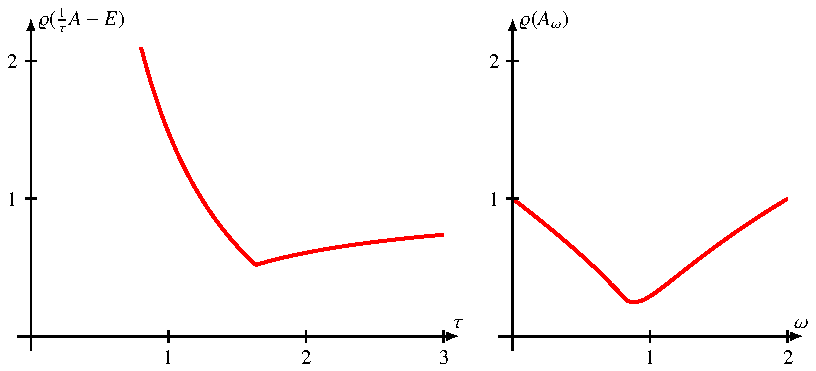
\includegraphics{chapters/60-linsys/images/sp.pdf}
\caption{Spektralradius für das Richardson-Verfahren in Abhängigkeit
von $\tau$ und für SOR in Abhängigkeit von $\omega$.
In beiden Fällen gibt es einen Parameterwert, für den die
Konvergenzgeschwindigkeit maximal ist.
\label{buch:figure:spektralradius}}
\end{figure}%
In Abbildung~\ref{buch:figure:spektralradius}
ist der Spektralradius der Iterationsmatrix für
das Richardson-Verfahren und für SOR dargestellt.
In beiden Fällen gibt es einen Wert für den Parameter,
für den der Spektralradius minimal und damit die Konvergenzgeschwindigkeit
am grössten wird.
\index{Konvergenzgeschwindigkeit}%
Es stellt sich heraus, dass das SOR-Verfahren in diesem speziellen Fall
für ein $\omega<1$ am schnellsten konvergiert, also für Unterrelaxation.
\end{beispiel}




%
% kondition.tex
%
% (c) 2020 Prof Dr Andreas Müller, Hochschule Rapperswil
%
\section{Kondition
\label{buch:section:kondition}}
Die Diskussion der iterativen Verfahren in
Abschnitt~\ref{buch:section:gaussseidel} hat gezeigt, dass
der Spektralradius aus Definition~\ref{buch:definition:spektralradius}
Auskunft gibt darüber, ob ein iteratives Verfahren konvergiert.
\index{Spektralradius}%
Insbesondere wurde behauptet, dass Spektralradius $\varrho(M)$ und
Gelfand-Radius $\pi(M)$ übereinstimmen.
In diesem Abschnitt sollen diese Kennzahl noch etwas vertieft
untersucht werden.

%
% Gelfand-Radius und Eigenwerte
%
\subsection{Gelfand-Radius und Eigenwerte
\label{buch:subsection:spektralradius}}
In Abschnitt~\ref{buch:subsection:konvergenzbedingung}
ist der Gelfand-Radius mit Hilfe eines Grenzwertes definiert worden.
\index{Gelfand-Radius}%
Nur dieser Grenzwert ist in der Lage, über die Konvergenz eines 
Iterationsverfahrens Auskunft zu geben.
Der Grenzwert ist aber sehr mühsam zu berechnen.
\index{Grenzwert}%
Es wurde angedeutet, dass der Gelfand-Radius mit dem Spektralradius
übereinstimmt, dem Betrag des des betragsgrössten Eigenwertes.
Dies hat uns ein vergleichsweise einfach auszuwertendes Konvergenzkriterium
geliefert.
\index{Konvergenzkriterium}%
In diesem Abschnitt soll diese Identität zunächst an Spezialfällen
und später ganz allgemein gezeigt werden.

\subsubsection{Spezialfall: Diagonalisierbare Matrizen}
Ist eine Matrix $A$ diagonalisierbar, dann kann Sie durch eine Wahl
einer geeigneten Basis in Diagonalform
\index{diagonalisierbar}%
\index{Diagonalform}%
\[
A'
=
\begin{pmatrix}
\lambda_1&        0&\dots &0\\
0        &\lambda_2&\dots &0\\
\vdots   &         &\ddots&\vdots\\
0        &        0&\dots &\lambda_n
\end{pmatrix}
\]
gebracht werden, wobei die Eigenwerte $\lambda_i$  möglicherweise auch
komplex sein können.
\index{komplex}%
Die Bezeichnungen sollen so gewählt sein, dass $\lambda_1$ der
betragsgrösste Eigenwert ist, dass also
\[
|\lambda_1| \ge |\lambda_2| \ge \dots \ge |\lambda_n|.
\]
Wir nehmen für die folgende, einführende Diskussion ausserdem an, dass
sogar $|\lambda_1|>|\lambda_2|$ gilt.

Unter den genannten Voraussetzungen kann man jetzt den Gelfand-Radius
von $A$ berechnen.
Dazu muss man $|A^nv|$ für einen beliebigen Vektor $v$ und für
beliebiges $n$ berechnen.
Der Vektor $v$ lässt sich in der Eigenbasis von $A$ zerlegen, also
als Summe
\index{Eigenbasis}%
\[
v = v_1+v_2+\dots+v_n
\]
schreiben, wobei $v_i$ Eigenvektoren zum Eigenwert $\lambda_i$ sind oder
Nullvektoren.
Die Anwendung von $A^k$ ergibt dann
\[
A^k v
=
A^k v_1 + A^k v_2 + \dots + A^k v_n
=
\lambda_1^k v_1 + \lambda_2^k v_2 + \dots + \lambda_n^k v_n.
\]
Für den Grenzwert braucht man die Norm von $A^kv$, also
\begin{align}
|A^kv|
&= |\lambda_1^k v_1 + \lambda_2^k v_2 + \dots + \lambda_3 v_3|
\notag
\\
\Rightarrow\qquad
\frac{|A^kv|}{\lambda_1^k}
&=
\biggl|
v_1 +
\biggl(\frac{\lambda_2}{\lambda_1}\biggr)^k v_2
+
\dots
+
\biggl(\frac{\lambda_n}{\lambda_1}\biggr)^k v_n
\biggr|.
\label{buch:spektralradius:eqn:eigenwerte}
\end{align}
Da alle Quotienten $|\lambda_i/\lambda_1|<1$ sind für $i\ge 2$,
konvergieren alle Terme auf der rechten Seite von
\eqref{buch:spektralradius:eqn:eigenwerte}
ausser dem ersten gegen $0$.
Folglich ist
\[
\lim_{k\to\infty} \frac{|A^kv|}{|\lambda_1|^k}
=
|v_1|
\qquad\Rightarrow\qquad
\lim_{k\to\infty} \frac{|A^kv|^\frac1k}{|\lambda_1|}
=
\lim_{k\to\infty}|v_1|^{\frac1k}
=
1.
\]
Dies gilt für alle Vektoren $v$, für die $v_1\ne 0$ ist.
Der maximale Wert dafür wird erreicht, wenn man für 
$v$ einen Eigenvektor der Länge $1$ zum Eigenwert $\lambda_1$ einsetzt,
dann ist $v=v_1$.
Es folgt dann
\[
\pi(A)
=
\lim_{k\to\infty} \| A^k\|^\frac1k
=
\lim_{k\to\infty} |A^kv|^\frac1k
=
|\lambda_1|
=
\varrho(A).
\]
Damit ist gezeigt, dass im Spezialfall einer diagonalisierbaren Matrix der
Gelfand-Radius tatsächlich der Betrag des betragsgrössten Eigenwertes ist.
\index{Gelfand-Radius}%

\subsubsection{Blockmatrizen}
Wir betrachten jetzt eine $(n+m)\times(n+m)$-Blockmatrix der Form
\begin{equation}
A = \begin{pmatrix} B & 0 \\ 0 & C\end{pmatrix}
\label{buch:spektralradius:eqn:blockmatrix}
\end{equation}
mit einer $n\times n$-Matrix $B$ und einer $m\times m$-Matrix $C$.
Ihre Potenzen haben ebenfalls Blockform:
\[
A^k = \begin{pmatrix} B^k & 0 \\ 0 & C^k\end{pmatrix}.
\]
Ein Vektor $v$ kann in die zwei Summanden $v_1$ bestehen aus den
ersten $n$ Komponenten und $v_2$ bestehen aus den letzten $m$ 
Komponenten zerlegen.
Dann ist
\[
A^kv = B^kv_1 + C^kv_2.
\qquad\Rightarrow\qquad
|A^kv|
\le
|B^kv_1| + |C^kv_2|
\le 
\pi(B)^k |v_1| + \pi(C)^k |v_2|.
\]
Insbesondere haben wir das folgende Lemma gezeigt:

\begin{lemma}
\label{buch:spektralradius:lemma:diagonalbloecke}
Eine diagonale Blockmatrix $A$ \eqref{buch:spektralradius:eqn:blockmatrix}
Blöcken $B$ und $C$  hat Gelfand-Radius
\[
\pi(A) = \max ( \pi(B), \pi(C) )
\]
\end{lemma}

Selbstverständlich lässt sich das Lemma auf Blockmatrizen mit beliebig
vielen diagonalen Blöcken verallgemeinern.
\index{Blockmatrix}%

Für Diagonalmatrizen der genannten Art sind aber auch die 
Eigenwerte leicht zu bestimmen.
\index{Diagonalmatrix}%
Hat $B$ die Eigenwerte $\lambda_i^{(B)}$ mit $1\le i\le n$ und $C$ die
Eigenwerte $\lambda_j^{(C)}$ mit $1\le j\le m$, dann ist das charakteristische
Polynom der Blockmatrix $A$ natürlich
\index{charakteristisches Polynom}%
\index{Polynom!charakteristisch}%
\[
\chi_A(\lambda) = \chi_B(\lambda)\chi_C(\lambda),
\]
woraus folgt, dass die Eigenwerte von $A$ die Vereinigung der Eigenwerte
von $B$ und $C$ sind.
Daher gilt auch für die Spektralradius die Formel
\[
\varrho(A) = \max(\varrho(B) , \varrho(C)).
\]

\subsubsection{Jordan-Blöcke}
\index{Jordan-Block}%
Nicht jede Matrix ist diagonalisierbar, die bekanntesten Beispiele sind
die Matrizen
\begin{equation}
J_n(\lambda)
=
\begin{pmatrix}
\lambda &      1&       &       &       &       \\
        &\lambda&      1&       &       &       \\[-5pt]
        &       &\lambda&\ddots &       &       \\[-5pt]
        &       &       &\ddots &      1&       \\
        &       &       &       &\lambda&      1\\
        &       &       &       &       &\lambda
\end{pmatrix},
\label{buch:spektralradius:eqn:jordan}
\end{equation}
wobei $\lambda\in\mathbb C$ eine beliebige komplexe Zahl ist.
Wir nennen diese Matrizen {\em Jordan-Matrizen}.
Es ist klar, dass $J_n(\lambda)$ nur den $n$-fachen Eigenwert
$\lambda$ hat und dass der erste Standardbasisvektor ein
Eigenvektor zu diesem Eigenwert ist.

In der linearen Algebra lernt man, dass jede Matrix durch Wahl
\index{lineare!Algebra}%
einer geeigneten Basis als Blockmatrix der Form
\[
A
=
\begin{pmatrix}
J_{n_1}(\lambda_1) &        0         & \dots & 0 \\
       0         & J_{n_2}(\lambda_2) & \dots & 0 \\[-4pt]
\vdots           &\vdots            &\ddots &\vdots \\
       0         &        0         & \dots &J_{n_l}(\lambda_l)
\end{pmatrix}
\]
geschrieben werden kann\footnote{Sofern die Matrix komplexe Eigenwerte
hat muss man auch komplexe Basisvektoren zulassen.}.
Die früheren Beobachtungen über den Spektralradius und den
Gelfand-Radius von Blockmatrizen zeigen uns daher, dass
nur gezeigt werden muss, dass nur die Gleichheit des Gelfand-Radius
und des Spektral-Radius von Jordan-Blöcken gezeigt werden muss.

\subsubsection{Iterationsfolgen}
\begin{satz}
\label{buch:spektralradius:satz:grenzwert}
Sei $A$ eine $n\times n$-Matrix mit Spektralradius $\varrho(A)$.
Dann ist $\varrho(A)<1$ genau dann, wenn
\[
\lim_{k\to\infty} A^k = 0.
\]
Ist andererseits $\varrho(A) > 1$, dann ist
\[
\lim_{k\to\infty} \|A^k\|=\infty.
\]
\end{satz}

\begin{proof}[Beweis]
Wie bereits angedeutet reicht es, diese Aussagen für einen einzelnen
Jordan-Block mit Eigenwert $\lambda$ zu beweisen.
Die $k$-te Potenz von $J_n(\lambda)$ ist
\[
J_n(\lambda)^k
=
\renewcommand\arraystretch{1.35}
\begin{pmatrix}
\lambda^k    & \binom{k}{1} \lambda^{k-1} & \binom{k}{2}\lambda^{k-2}&\dots&
\binom{k}{n-1}\lambda^{k-n+1}\\
      0      &\lambda^k & \binom{k}{1} \lambda^{k-1} & \dots &\binom{k}{n-2}\lambda^{k-n+2}\\
      0     &      0    & \lambda^k & \dots &\binom{k}{n-k+3}\lambda^{k-n+3}\\
\vdots      & \vdots    &               &\ddots & \vdots\\
     0      &      0    &      0        &\dots  &\lambda^k
\end{pmatrix}.
\]
Falls $|\lambda| < 1$ ist, gehen alle Potenzen von $\lambda$ exponentiell
schnell gegen $0$, während die Binomialkoeffizienten nur polynomiell
schnell anwachsen. 
\index{Binomialkoeffizient}
In diesem Fall folgt also $J_n(\lambda)\to 0$.

Falls $|\lambda| >1$ divergieren bereits die Elemente auf der Diagonalen,
also ist $\|J_n(\lambda)^k\|\to\infty$ mit welcher Norm auch immer man
man die Matrix misst.
\end{proof}

Aus dem Beweis kann man noch mehr ablesen.
Für $\varrho(A)< 1$ ist die Norm $ \|A^k\| \le M \varrho(A)^k$ für eine
geeignete Konstante $M$,
für $\varrho(A) > 1$ gibt es eine Konstante $m$ mit
$\|A^k\| \ge m\varrho(A)^k$.

\subsubsection{Der Satz von Gelfand}
Der Satz von Gelfand ergibt sich jetzt als direkte Folge aus dem
Satz~\ref{buch:spektralradius:satz:grenzwert}.

\begin{satz}[Gelfand]
\index{Satz von Gelfand}
\index{Gelfand!Satz von}
\label{buch:satz:gelfand}
Für jede komplexe $n\times n$-Matrix $A$ gilt
\[
\pi(A)
=
\lim_{k\to\infty}\|A^k\|^\frac1k
=
\varrho(A).
\]
\end{satz}

\begin{proof}[Beweis]
Der Satz~\ref{buch:spektralradius:satz:grenzwert} zeigt, dass der
Spektralradius ein scharfes Kriterium dafür ist, ob $\|A^k\|$ 
gegen 0 oder $\infty$ konvergiert.
Andererseits ändert ein Faktor $t$ in der Matrix $A$ den Spektralradius
ebenfalls um den gleichen Faktor, also $\varrho(tA)=t\varrho(A)$.
Natürlich gilt auch
\[
\pi(tA)
=
\lim_{k\to\infty} \|t^kA^k\|^\frac1k
=
\lim_{k\to\infty} t\|A^k\|^\frac1k
=
t\lim_{k\to\infty} \|A^k\|^\frac1k
=
t\pi(A).
\]

Wir betrachten jetzt die Matrix
\[
A(\varepsilon) = \frac{A}{\varrho(A) + \varepsilon}.
\]
Der Spektralradius von $A(\varepsilon)$ ist
\[
\varrho(A(\varepsilon)) = \frac{\varrho(A)}{\varrho(A)+\varepsilon},
\]
er ist also $>1$ für negatives $\varepsilon$ und $<1$ für positives
$\varepsilon$.
Aus dem Satz~\ref{buch:spektralradius:satz:grenzwert} liest man daher ab,
dass $\|A(\varepsilon)^k\|$ genau dann gegen $0$ konvergiert, wenn
$\varepsilon > 0$ ist und divergiert genau dann, wenn $\varepsilon< 0$ ist.

Aus der Bemerkung nach dem Beweis von
Satz~\ref{buch:spektralradius:satz:grenzwert} schliesst man daher, dass 
es im Fall $\varepsilon > 0$ eine Konstante $M$ gibt mit
\begin{align*}
\|A(\varepsilon) ^k\|\le M\varrho(A(\varepsilon))^k
\quad&\Rightarrow\quad
\|A(\varepsilon) ^k\|^\frac1k\le M^\frac1k\varrho(A(\varepsilon))
\\
&\Rightarrow\quad
\pi(A) \le  \varrho(A(\varepsilon))
\underbrace{\lim_{k\to\infty} M^\frac1k}_{\displaystyle=1}
=
\varrho(A(\varepsilon))
=
\varrho(A)+\varepsilon.
\end{align*}
Dies gilt für beliebige $\varepsilon >0$, es folgt daher
$\pi(A) \le \varrho(A)$.

Andererseits gibt es für $\varepsilon <0$ eine Konstante $m$ mit
\begin{align*}
\|A(\varepsilon) ^k\|\ge m\varrho(A(\varepsilon))^k
\quad&\Rightarrow\quad
\|A(\varepsilon) ^k\|^\frac1k\ge m^\frac1k\varrho(A(\varepsilon))
\\
&\Rightarrow\quad
\pi(A) \ge  \varrho(A(\varepsilon))
\underbrace{\lim_{k\to\infty} m^\frac1k}_{\displaystyle=1}
=
\varrho(A(\varepsilon))
=
\varrho(A)+\varepsilon.
\end{align*}
Dies gilt für beliebige $\varepsilon> 0$, es folgt daher
$\pi(A) \ge \varrho(A)$.
Zusammen mit $\pi(A) \le \varrho(A)$ folgt $\pi(A)=\varrho(A)$.
\end{proof}

%
% Konditionszahl
%
\subsection{Konditionszahl
\label{buch:subsection:konditionszahl}}
\index{Konditionszahl}%
Der Spektralradius $\varrho(A)$ einer Matrix $A$ gibt darüber Auskunft,
ob ein auf $A$ basierendes Iterationsverfahren konvergiert.
Er sagt aber nicht einmal, ob die Matrix zum Beispiel regulär.
Doch auch diese Information lässt sich aus den Eigenwerten ablesen.
Die Matrix ist genau dann regulär, wenn alle Eigenwerte von $0$ verschieden
sind.
Ein Problem entsteht also dann, wenn einzelne Eigenwerte sehr klein sind.
Die Kombination besonders grosser und besonders kleiner Eigenwerte 
ist also ein Indikator, der auf mögliche numerische Probleme hinweisen kann.

Die Eigenwerte von $A^{-1}$ sind die Reziproken der Eigenwerte von $A$.
Ist $\lambda$ ein Eigenwert von $A$, dann ist $\lambda^{-1}$ ein Eigenwert
von $A^{-1}$.
Der betragskleinste Eigenwert von $A$ ist der betragsgrösste Eigenwert von
$A^{-1}$.
Numerische Probleme werden also dadurch angezeigt, dass $\varrho(A)$ gross
ist, oder $\varrho(A^{-1})$ klein.

\begin{definition}
\label{buch:konditionszahl:definition}
\index{Konditionszahl}%
Die Konditionszahl einer Matrix $A$ ist der Quotient
\[
\kappa(A)
=
\frac{\varrho(A)}{\varrho(A^{-1})}
=
\frac{|\lambda_1|}{|\lambda_n|},
\]
wenn $\lambda_1$ der betragsgrösste und $\lambda_n$ der betragskleinste
Eigenwert von $A$ ist.
\end{definition}

Die Konditionszahl ist also immer $\ge 1$, dieser minimale Wert $1$
wird zum Beispiel für die Einheitsmatrix erreicht.
Schlechte Kondition tritt auf, wenn die Eigenwerte sehr grosse
Betragsunterschiede aufweisen.
\index{Kondition!schlecht}

\begin{beispiel}
Die Kahan-Matrix
\index{Kahan-Matrix}%
\[
A
=
\begin{pmatrix}
1000&999\\
999&998
\end{pmatrix}
\]
besteht aus zwei fast gleichen Zeilen, sie ist als fast singulär,
die Determinante muss sehr klein sein.
Andererseits sind alle Einträge von der Grössenordnung $10^3$, man erwartet
also einen Spektralradius in der selben Grössenordnung.
Die Konditionszahl dürfte daher weit grösser als $10^3$ sein.
Die numerische Rechnung ergibt für die Eigenwerte
\[
\lambda_1 = 1998.00050050375,
\qquad
\lambda_2 = -0.000500500375,
\]
was eine Konditionszahl von
\[
\kappa(A)
\approx
3992006
\approx
4\cdot 10^6
\]
ergibt.
Diese einfache Matrix hat also sehr schlechte Kondition.

Die Determinante von $A$ ist
\index{Determinante}%
\[
\det A
=
1000\cdot 998 -999^2
=
-1.
\]
Damit kann man auch die Inverse algebraisch leicht angeben:
\index{Inverse}%
\[
A^{-1}
=
\frac{1}{\det(A)}
\begin{pmatrix} 998 & -999\\ -999 &1000 \end{pmatrix}.
\]
Die numerische Rechnung offenbart aber die Schwierigkeiten, die die 
schlechte Kondition verursacht.
Das Produkt $AA^{-1}$ müsste die Einheitsmatrix ergeben, die numerische
Rechnung mit dem \texttt{double}-Typ ergibt jedoch
\[
\begin{pmatrix}
   1.0000000000{\color{red}74920} &-0.0000000000{\color{red}52182}\\
   0.00000000000{\color{red}3410} &\phantom{-}1.0000000000{\color{red}20236}
\end{pmatrix},
\]
der numerische Fehler ist also etwa um den Faktor $10^4$ grösser als
bei einer gut konditionierten Matrix erwartet werden kann.
\end{beispiel}



%
% qr.tex
%
% (c) 2020 Prof Dr Andreas Müller, Hochschule Rapperswil
%
\section{QR-Zerlegung mit Spiegelungen
\label{buch:section:qr}}
\rhead{QR-Zerlegung mit Spiegelungen}
\index{QR-Zerlegung}%
Das Orthonormalisierungsproblem verlangt, dass zu gegebenen Vektoren
$a_1,\dots,a_n\in \mathbb R^l$ orthonormierte Vektoren $q_1,\dots ,q_n$
gefunden werden derart, dass
\begin{equation}
a_k
=
\langle q_1,\dots,q_k \rangle
\qquad
\forall 1\le k\le n.
\label{buch:eqn:qr:span}
\end{equation}
Die Bedingung \eqref{buch:eqn:qr:span} bedeutet, dass es Zahlen $r_{ik}$
mit $i\le k$ derart, dass
\begin{equation}
a_k = q_1 r_{11} +  q_2 r_{12} + \dots + q_k r_{1k}
\label{buch:eqn:qr:span2}
\end{equation}
Schreiben wir die Komponenten des Vektors $a_k$ als $l\times n$-Matrix
$A$ mit Einträgen $a_{ik}$ und analog für die Vektoren $q_k$, dann kann
\eqref{buch:eqn:qr:span2} in Matrixform geschrieben werden als
\[
A=QR, \qquad\text{mit}\quad
R
=
\begin{pmatrix}
r_{11}&r_{12}&\dots &r_{1n}\\
0     &r_{22}&\dots &r_{2n}\\
0     &0     &\dots &r_{3n}\\
\vdots&\vdots&\ddots&\vdots\\
\end{pmatrix}
\]
Darin ist $Q$ eine $l\times n$-Matrix und $R$ ist eine $n\times n$-Matrix.
Die Aufgabe, eine Menge von Vektoren $\{a_1,\dots,a_n\}$ zu orthonormieren,
ist also gleichbedeutend damit, für die Matrix $A$ eine Zerlegung $A=QR$
zu finden, wobei $Q$ orthogonal und $R$ eine obere Dreiecksmatrix sein soll.
\index{Dreiecksmatrix}%

%
% Gram-Schmidt-Orthonormalisierung
%
\subsection{Gram-Schmidt-Orthonormalisierung
\label{buch:subsection:gram-schmidt}}
Das einfachste und anschaulichste Orthonormalisierungsverfahren, der
Gram-Schmidt-Prozess verwendet die Formeln
\index{Gram-Schmidt-Prozess}%
\begin{align*}
q_1 & = \frac{a_1}{|a_1|}
\\
q_2 &= \frac{
a_2 - (q_1\cdot a_2) q_1
}{
|a_2 - (q_1\cdot a_2) q_1|
}
\\
q_3 &= \frac{
a_3 - (q_1\cdot a_3) q_1 - (q_2\cdot a_3) q_2
}{
|a_3 - (q_1\cdot a_3) q_1 - (q_2\cdot a_3) q_2|
}
\\
&\;\vdots\\
q_k
&=\frac{
a_k - (q_1\cdot a_k) q_1 -\dots- (q_{k-1}\cdot a_k) q_{k-1}
}{|
a_k - (q_1\cdot a_k) q_1 -\dots- (q_{k-1}\cdot a_k) q_{k-1}
|},
\end{align*}
um die orthonormierten Vektoren $q_k$ zu finden.
\index{orthonormiert}%
Wegen der Differenzen im Zähler und Nenner besteht die Gefahr von
Auslöschung, falls der Winkel zwischen $a_k$ und
$\langle a_1,\dots,a_{k-1}\rangle$ sehr klein ist.
\index{Auslöschung}%
Der Gram-Schmidt-Prozess ist daher in seiner Grundform nicht immer stabil.
In Kapitel~\ref{chapter:qr} wird an einem Simulationsbeispiel gezeigt,
wie sich die Instabilität des Gram-Schmidt-Algorithmus äusseren kann.

\subsection{Spiegelungen
\label{buch:subsection:spiegelungn}}
Mit dem Skalarprodukt kann zu jedem Paar $a$, $b$ von Vektoren 
gleicher Länge eine Matrix gefunden werden, welche eine Spiegelung
beschreibt, die $a$ auf $b$ abbildet, alle Vektoren orthogonal zu
$a$ und $b$ aber unverändert lässt.
\index{Skalarprodukt}%
\index{Spiegelung}%

Sei $n=(b-a)/|b-a|$ der Einheitsvektor in Richtung $b-a$.
Es ist $(a-b)\cdot (a+b) = |a|^2 - |b|^2$, also auch $n\cdot (a+b)=0$.
\index{Einheitsvektor}%

Die Abbildung
\[
s:
x\mapsto  x - 2 n(n\cdot x) 
\]
hält auf $n$ orthogonale Vektoren $x$ wegen $n\cdot x=0$ fest.
Für die Vektoren $a$ und $b$ ist $(b-a)\cdot a= -(b-a)\cdot b$, so
dass
\begin{align*}
a
&=
\underbrace{\frac12(a+b)}_{\displaystyle =u}
+
\underbrace{\frac12(a-b)}_{\displaystyle=v}
=
u+v
\\
b&= \frac12(a+b) - \frac12(a-b) = u - v
\end{align*}
gilt mit orthogonalen Vektoren $u=\frac12(a+b)$ und $v=\frac12(a-b)$.
Für die beiden Summanden gilt
\begin{align*}
s(u) &= u,\\
s(v) &= -v
\end{align*}
und daher
\begin{align*}
s(a)
&=
s(u+v)=s(u)+s(v)=u-v = b,
\\
s(b)
&=
s(u-v)=s(u)-s(v)=u+v = a.
\end{align*}
Die Abbildung $s$ vertauscht also die beiden Vektoren, sie ist eine
Spiegelung in der von $a$ und $b$ aufgespannten Ebene an einer
Geraden mit der Normalen $n$.

Der Vektor $n$ ermöglicht auch, die lineare Abbildung $s$ mit Hilfe
einer Matrix $s$ zu schreiben.
Das Skalarprodukt $n\cdot x$ ist das Matrixprodukt $n^t x$, der Vektor
$n(n\cdot x)$ als Matrixprodukt $nn^tx$ berechnet werden. 
Damit wird 
\[
s(x)
=
x - 2n(n\cdot x)
=
Ex - 2(nn^t) x
=
(E-2nn^t) x
\qquad\Rightarrow\qquad
S=E-2nn^t
\]
die Matrix der Abbildung $s$.
Wir haben damit den folgenden Satz bewiesen.

\begin{satz}
\label{buch:satz:sab}
Zu gegebenen Vektoren $a$ und $b$ gleicher, nicht verschwindender
Länge gibt es eine orthogonale Matrix
\[
S_{a,b} = E-2nn^t\qquad \text{mit}\quad n = (b-a)/|b-a|,
\]
die zu einer Spiegelung gehört, die $a$ auf $b$ abbildet und
umgekehrt  und ausserdem alle Vektoren senkrecht auf $a$ und $b$ fest lässt.
\end{satz}
\index{Spiegelungsmatrix}%

%
% QR-Zerlegung mit Spiegelungen
%
\subsection{QR-Zerlegung mit Spiegelungen
\label{buch:subsection:qrspiegelungen}}
Aus der QR-Zerlegung $A=QR$ erhält man durch Multiplikation mit $Q^t$
die Gleichung $Q^tA=R$.
Die Aufgabe, die QR-Zerlegung zu finden, ist also gleichbedeutend damit,
eine Matrix durch Multiplizieren mit orthogonalen Matrizen auf Dreiecksform
zu bringen.
\index{QR-Zerlegung}%
Das Produkt der orthogonalen Matrizen ist $Q^t$.
In diesem Abschnitt wird ein Algorithmus basierend auf den Matrizen
$S_{a,b}$ vorgestellt, der genau dies leistet.

Sei $a\in\mathbb R^l$ ein nicht verschwindender Vektor.
Dann ist der Vektor $b=(|a|,0,\dots,0)^t$ ein Vektor gleicher Länge.
Nach Satz~\ref{buch:satz:sab} ist die Matrix $S_{a,b}$ eine Spiegelung,
die $a$ auf $b$ abbildet.

Sei jetzt ein Vektor $a\in\mathbb R^l$ gegeben und eine Zahl $k< l$.
Wir zerlegen den Vektor $a$ in zwei Teile
\[
a = \begin{pmatrix}\tilde{a}\\\bar{a}\end{pmatrix}
\quad\text{mit}\quad
\tilde{a}=\begin{pmatrix}a_1\\\vdots\\a_{k-1}\end{pmatrix}
\bar{a}=\begin{pmatrix}a_k\\\vdots \\a_l\end{pmatrix}.
\]
Die Matrix $Q_{\bar{a}}$ bildet $\bar{a}$ auf einen Vektor ab, von dem
nur die erste Komponente von $0$ verschieden ist.
Daraus wird die Matrix
\begin{equation}
Q_a
=
\begin{pmatrix} E&0\\0&Q_{\bar{a}}\end{pmatrix},
\label{buch:eqn:Qa}
\end{equation}
die den Vektor
\[
a=\begin{pmatrix}
a_1\\\vdots\\ a_{k-1}\\a_{k}\\\vdots\\a_n
\end{pmatrix}
\qquad\text{auf}\qquad
Q_aa
=
\begin{pmatrix}a_1\\\vdots\\a_{k-1}\\ |\bar{a}|\\\vdots\\0\end{pmatrix}
\]
abbildet.
$Q_a$ lässt Vektoren $x$, für die $\bar{x}=0$ ist, unverändert.

Daraus lässt sich jetzt ein QR-Algorithmus konstruieren.

\begin{satz}[QR-Zerlegung mit Spiegelungen]
Gegeben ist die $l\times n$-Matrix $A$ mit $n\le l$.
Dann gibt es orthogonale Matrizen $Q_1,\dots,Q_n$ derart, dass in
jeder Matrix der Folge
\[
A_0 = A, \quad A_{i} = Q_{i}A_{i-1}\quad\text{für $0<i\le n$}
\]
die ersten $i$ Spalten die Form einer oberen Dreicksmatrix haben.
\index{Dreiecksmatrix}%
Mit $Q=Q_1^t\dots Q_n^t$ und $R=A_n=Q_n\dots Q_1A$ gilt $A=QR$.
\end{satz}

\begin{proof}[Beweis]
Wir müssen die Matrix $Q_i$ aus $A_{i-1}$ konstruieren.
Sei $a$ die $i$-te Matrix von $A_{i-1}$, dann setzen wir
$Q_i=Q_{a}$ mit der Matrix $Q_a$ nach \eqref{buch:eqn:Qa}.
Die Multiplikation mit $Q_i$ bringt die Spalte $i$ der Matrix 
$A_{i-1}$ in die für $A_{i}$ verlangte Form, ohne die 
Spalten mit Spaltenindex $<i$ zu verändern, da deren Komponenten dort,
wo $Q_a$ etwas bewirkt, alle verschwinden.
\end{proof}

\begin{beispiel}
Die Vektoren
\[
a_1 = \begin{pmatrix}1\\1\\1\end{pmatrix},
\qquad
a_2 = \begin{pmatrix}0\\1\\1\end{pmatrix},
\qquad
a_3 = \begin{pmatrix}0\\0\\1\end{pmatrix}
\]
sollen orthonormalisiert werden.
Die Matrix $Q_1$ spiegelt den Vektor 
\[
\begin{pmatrix}
1\\1\\1
\end{pmatrix}
\quad\text{auf}\quad
\begin{pmatrix}\sqrt{3}\\0\\0\end{pmatrix}
\]
ab.
Die zugehörige Matrix ist
\[
Q_1
=
\begin{pmatrix}
\frac{1}{\sqrt{3}} & \frac{1}{\sqrt{3}}          & \frac{1}{\sqrt{3}} \\
\frac{1}{\sqrt{3}} & \frac12-\frac{1}{2\sqrt{3}} & -\frac12-\frac{1}{2\sqrt{3}}\\
\frac{1}{\sqrt{3}} & -\frac12-\frac{1}{2\sqrt{3}}&\frac12-\frac1{2\sqrt{3}}
\end{pmatrix}
\qquad
A_1
=
Q_1A
=
\begin{pmatrix}
\sqrt{3} &  \frac{2}{\sqrt{3}} & \frac{1}{\sqrt{3}} \\
  0      & -\frac{1}{\sqrt{3}} & -\frac12-\frac{1}{2\sqrt{3}} \\
  0      & -\frac{1}{\sqrt{3}} & \frac12-\frac{1}{2\sqrt{3}}
\end{pmatrix}.
\]
Die zweite Matrix $Q_2$ ist
\[
Q_2
=
\begin{pmatrix}
1&0&0\\
0&-\frac{1}{\sqrt{2}} & -\frac{1}{\sqrt{2}} \\
0&-\frac{1}{\sqrt{2}} &  \frac{1}{\sqrt{2}}
\end{pmatrix},
\qquad
R
=
A_2 = Q_2A_1
=
\begin{pmatrix}
\sqrt{3} & \frac{2}{\sqrt{3}} & \frac{1}{\sqrt{3}} \\
    0    & \sqrt{\frac{2}{3}} & \frac{1}{\sqrt{6}} \\
    0    &         0          & \frac{1}{\sqrt{2}}
\end{pmatrix}
\]
Wegen $R=(Q_2Q_1)A$ folgt $A=(Q_2Q_1)^t R$ und damit
\[
Q=(Q_2Q_1)^t
=
\begin{pmatrix}
\frac{1}{\sqrt{3}} & - \sqrt{\frac{2}{3}} & 0\\
\frac{1}{\sqrt{3}} & \frac{1}{\sqrt{6}}   & - \frac{1}{\sqrt{2}} \\
\frac{1}{\sqrt{3}} & \frac{1}{\sqrt{6}}   & \frac{1}{\sqrt{2}}
\end{pmatrix}.
\]
Damit ist die QR-Zerlegung der Matrix $A$ gefunden.
Tatsächlich bilden die Spalten von $Q$ eine orthonormierte Basis
von $\mathbb R^3$, sie stimmt mit der Basis überein, die der
Gram-Schmidt-Prozess aus den Spalten der Matrix $A$ ableitet.
\index{Gram-Schmidt-Prozess}%
\end{beispiel}

Der Nachteil dieser Methode ist, dass die Matrizen $S_{a,b}$ typischerweise
sehr viele Einträge haben und dass damit die Matrixprodukte mit $S_{a,b}$
aufwendig zu berechnen sind.
Dies kann durch die Verwendung von Drehmatrizen, sogenannten Givens-Rotationen,
verbessert werden, wie dies in Kapitel~\ref{chapter:qr} durchgeführt wird.
\index{Drehmatrix}%
\index{Givens-Rotation}%


%
% jacobi.tex
%
% (c) 2020 Prof Dr Andreas Müller, Hochschule Rapperswil
%
\section{Jacobi-Verfahren
\label{buch:section:jacobi}}



\section*{Übungsaufgaben}
\rhead{Übungsaufgaben}
\aufgabetoplevel{chapters/60-linsys/uebungsaufgaben}
\begin{uebungsaufgaben}
\uebungsaufgabe{6002}
\uebungsaufgabe{6003}
\uebungsaufgabe{6001}
\end{uebungsaufgaben}




